

\section{Experimental Results and Discussion}

\subsection{AI Velocity Regressor Accuracy}

Table~\ref{tab:reg} reports regression performance of the standalone GBDT velocity regressor on normalized 1.0\,s temporal windows. The model achieves an $R^2$ of 0.9225 and an RMSE of 1.723\,m/s on the unseen held-out evaluation track, confirming generalization to previously unseen driving manoeuvres and road topography.

\begin{table}[h]
\caption{AI Velocity Regressor Performance}
\label{tab:reg}
\centering
\begin{tabular}{lccc}
\toprule
\textbf{Dataset} & \textbf{RMSE (m/s)} & \textbf{MAE (m/s)} & \textbf{$R^2$} \\
\midrule
Training Set (7,500 samples) & 0.798 & 0.561 & 0.9877 \\
Held-Out Track (3,000 samples) & 1.723 & 1.083 & 0.9225 \\
\bottomrule
\end{tabular}
\end{table}

\subsection{Quantitative Multi-Baseline Benchmark across GNSS Outages}

Table~\ref{tab:benchmark} provides a systematic comparison between Naive INS double integration, AI Speed Alone (unfiltered), the Proposed ESKF (IDR core), and the Full Proposed System (ESKF + 3D Map Matching) across simulated GNSS outages spanning 10\,s to 120\,s. Drift is reported both as \emph{absolute endpoint drift} (terminal displacement against ground truth, relative to distance travelled) and \emph{net accumulated drift rate} (pure drift accumulated strictly during the outage window, removing any pre-existing filter bias at outage onset).

\begin{figure}[h]
\centering
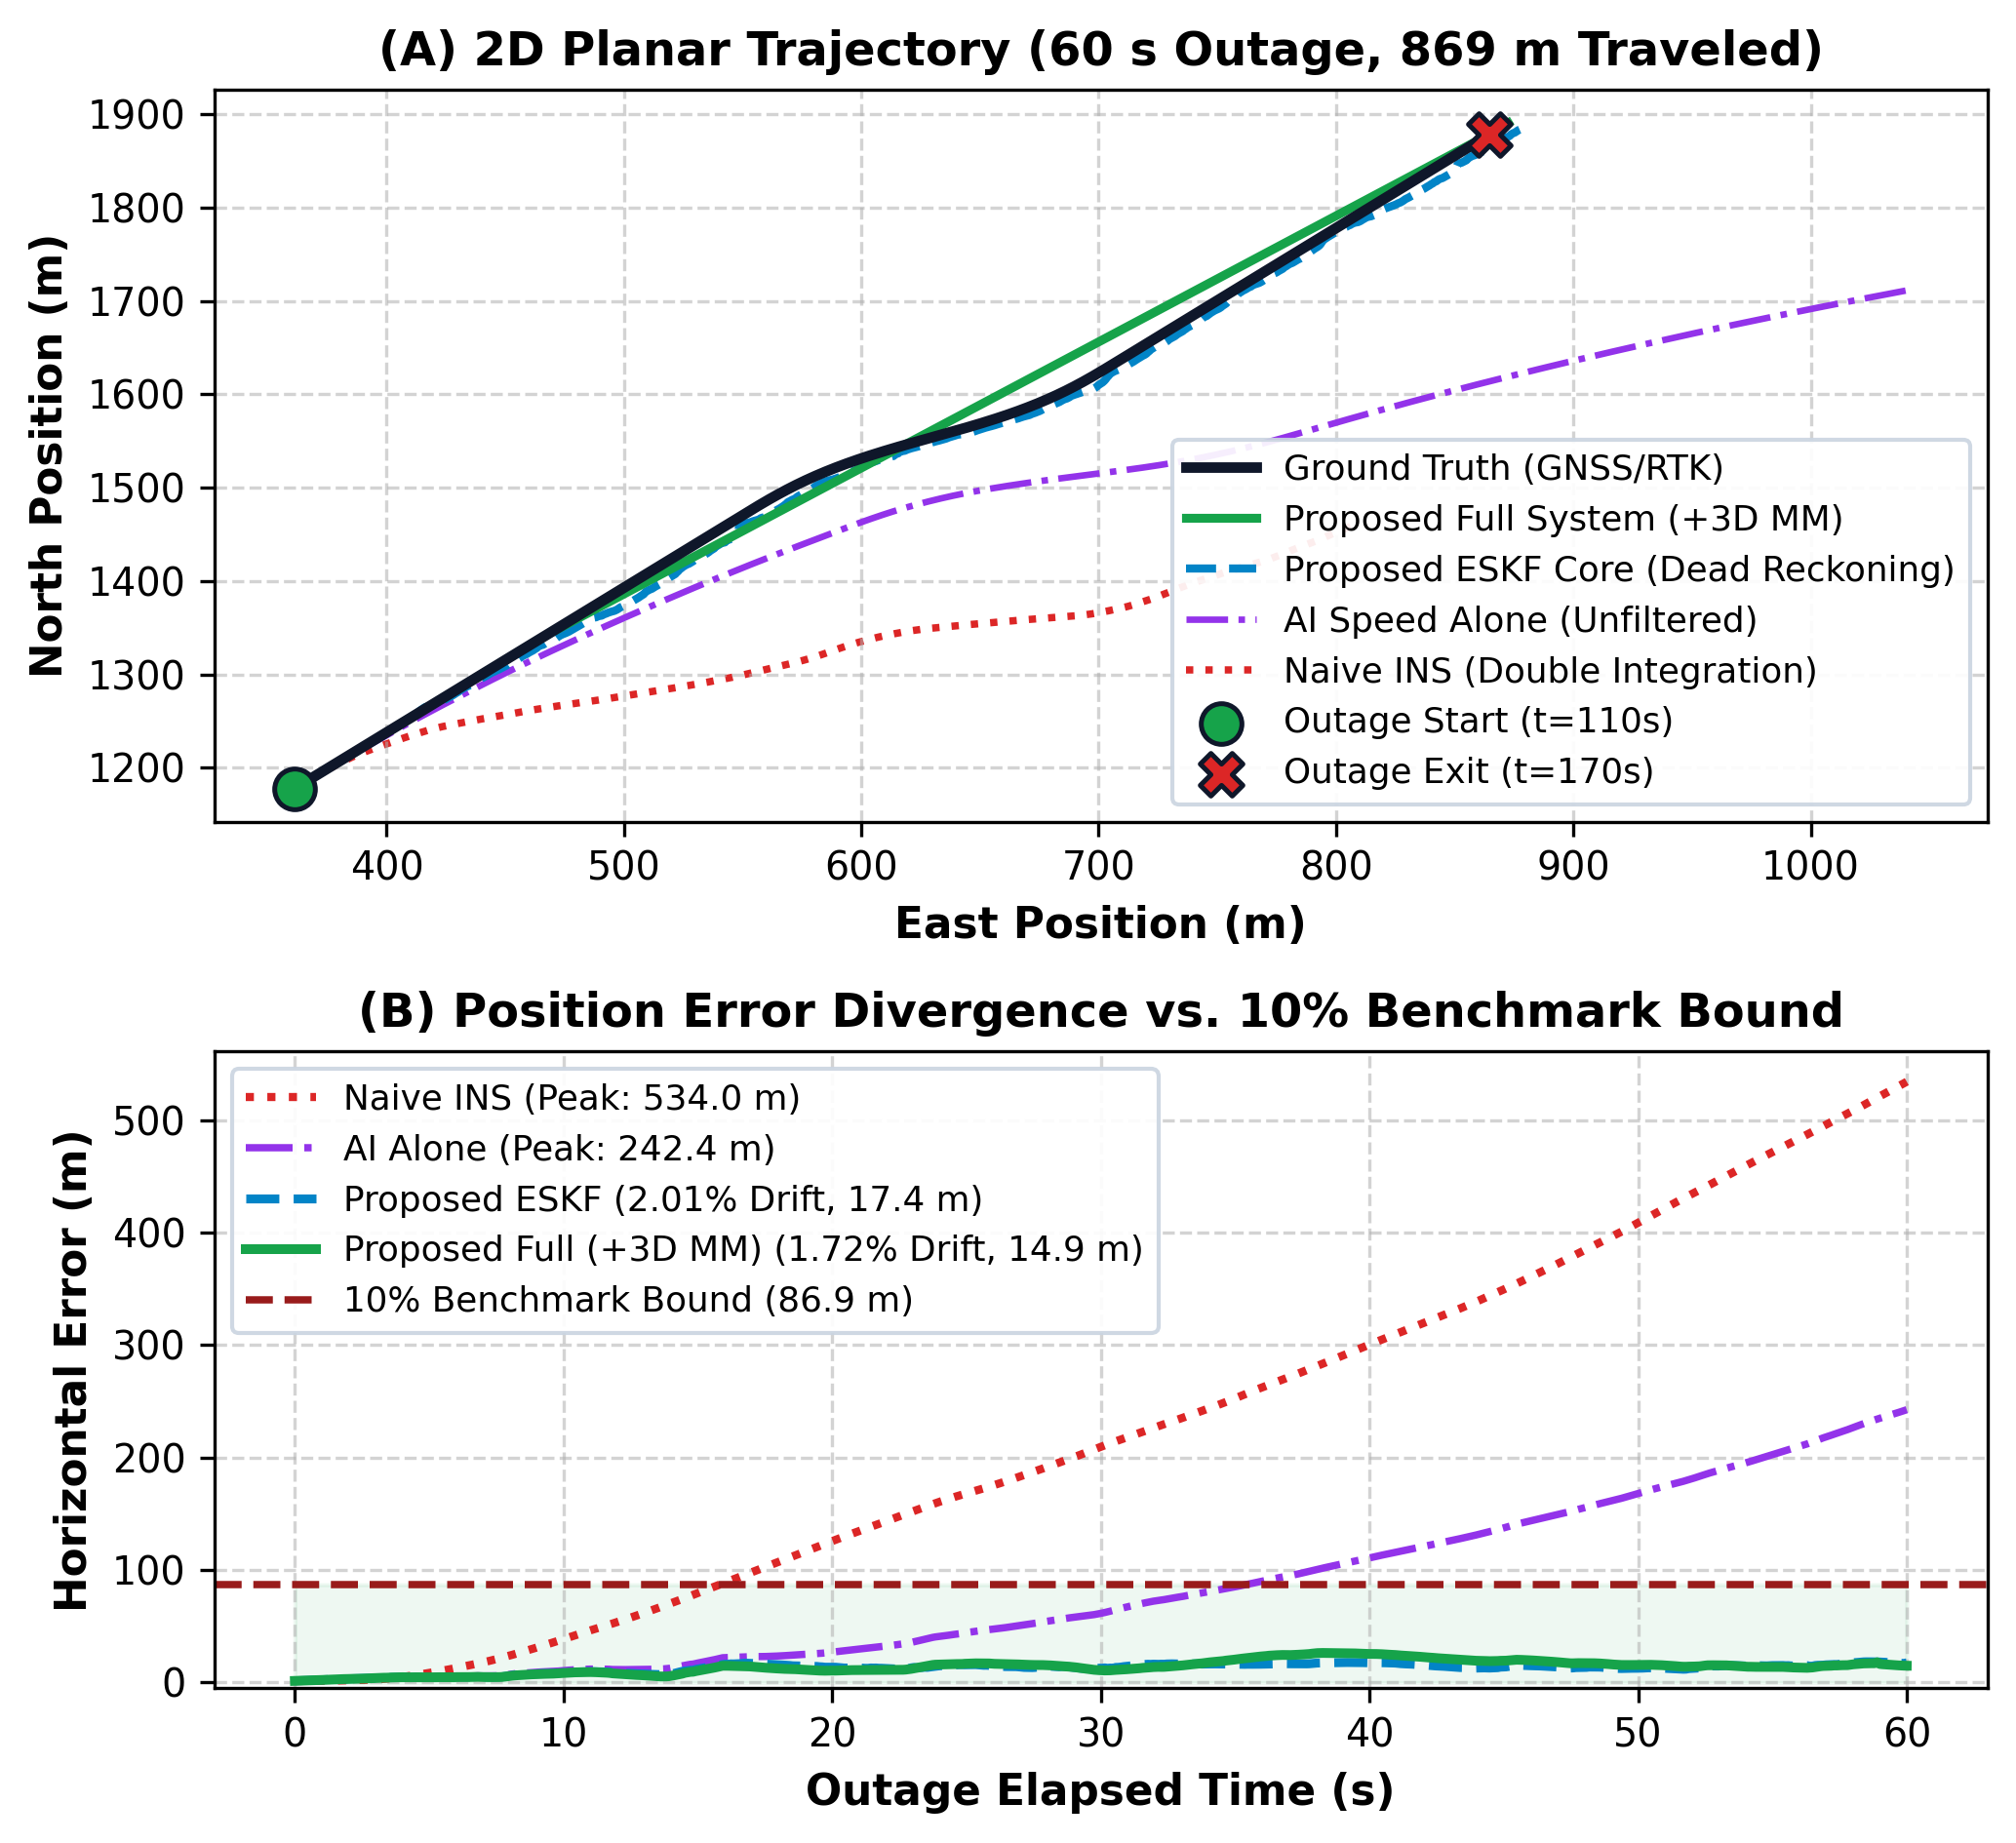
\includegraphics[width=\columnwidth]{fig_trajectory.png}
\caption{2D Planar Trajectory and Real-Time Position Error Divergence during a 60\,s GNSS outage (868.8\,m travel) across an elevated flyover. Naive integration diverges by 534.0\,m (max), AI-alone diverges by 242.4\,m (max), while the proposed ESKF tracks ground truth with a maximum error of 18.4\,m (2.01\% drift) and the full system (+3D MM) reaches 26.3\,m maximum error (1.72\% drift).}
\label{fig:traj}
\end{figure}

\begin{figure}[h]
\centering
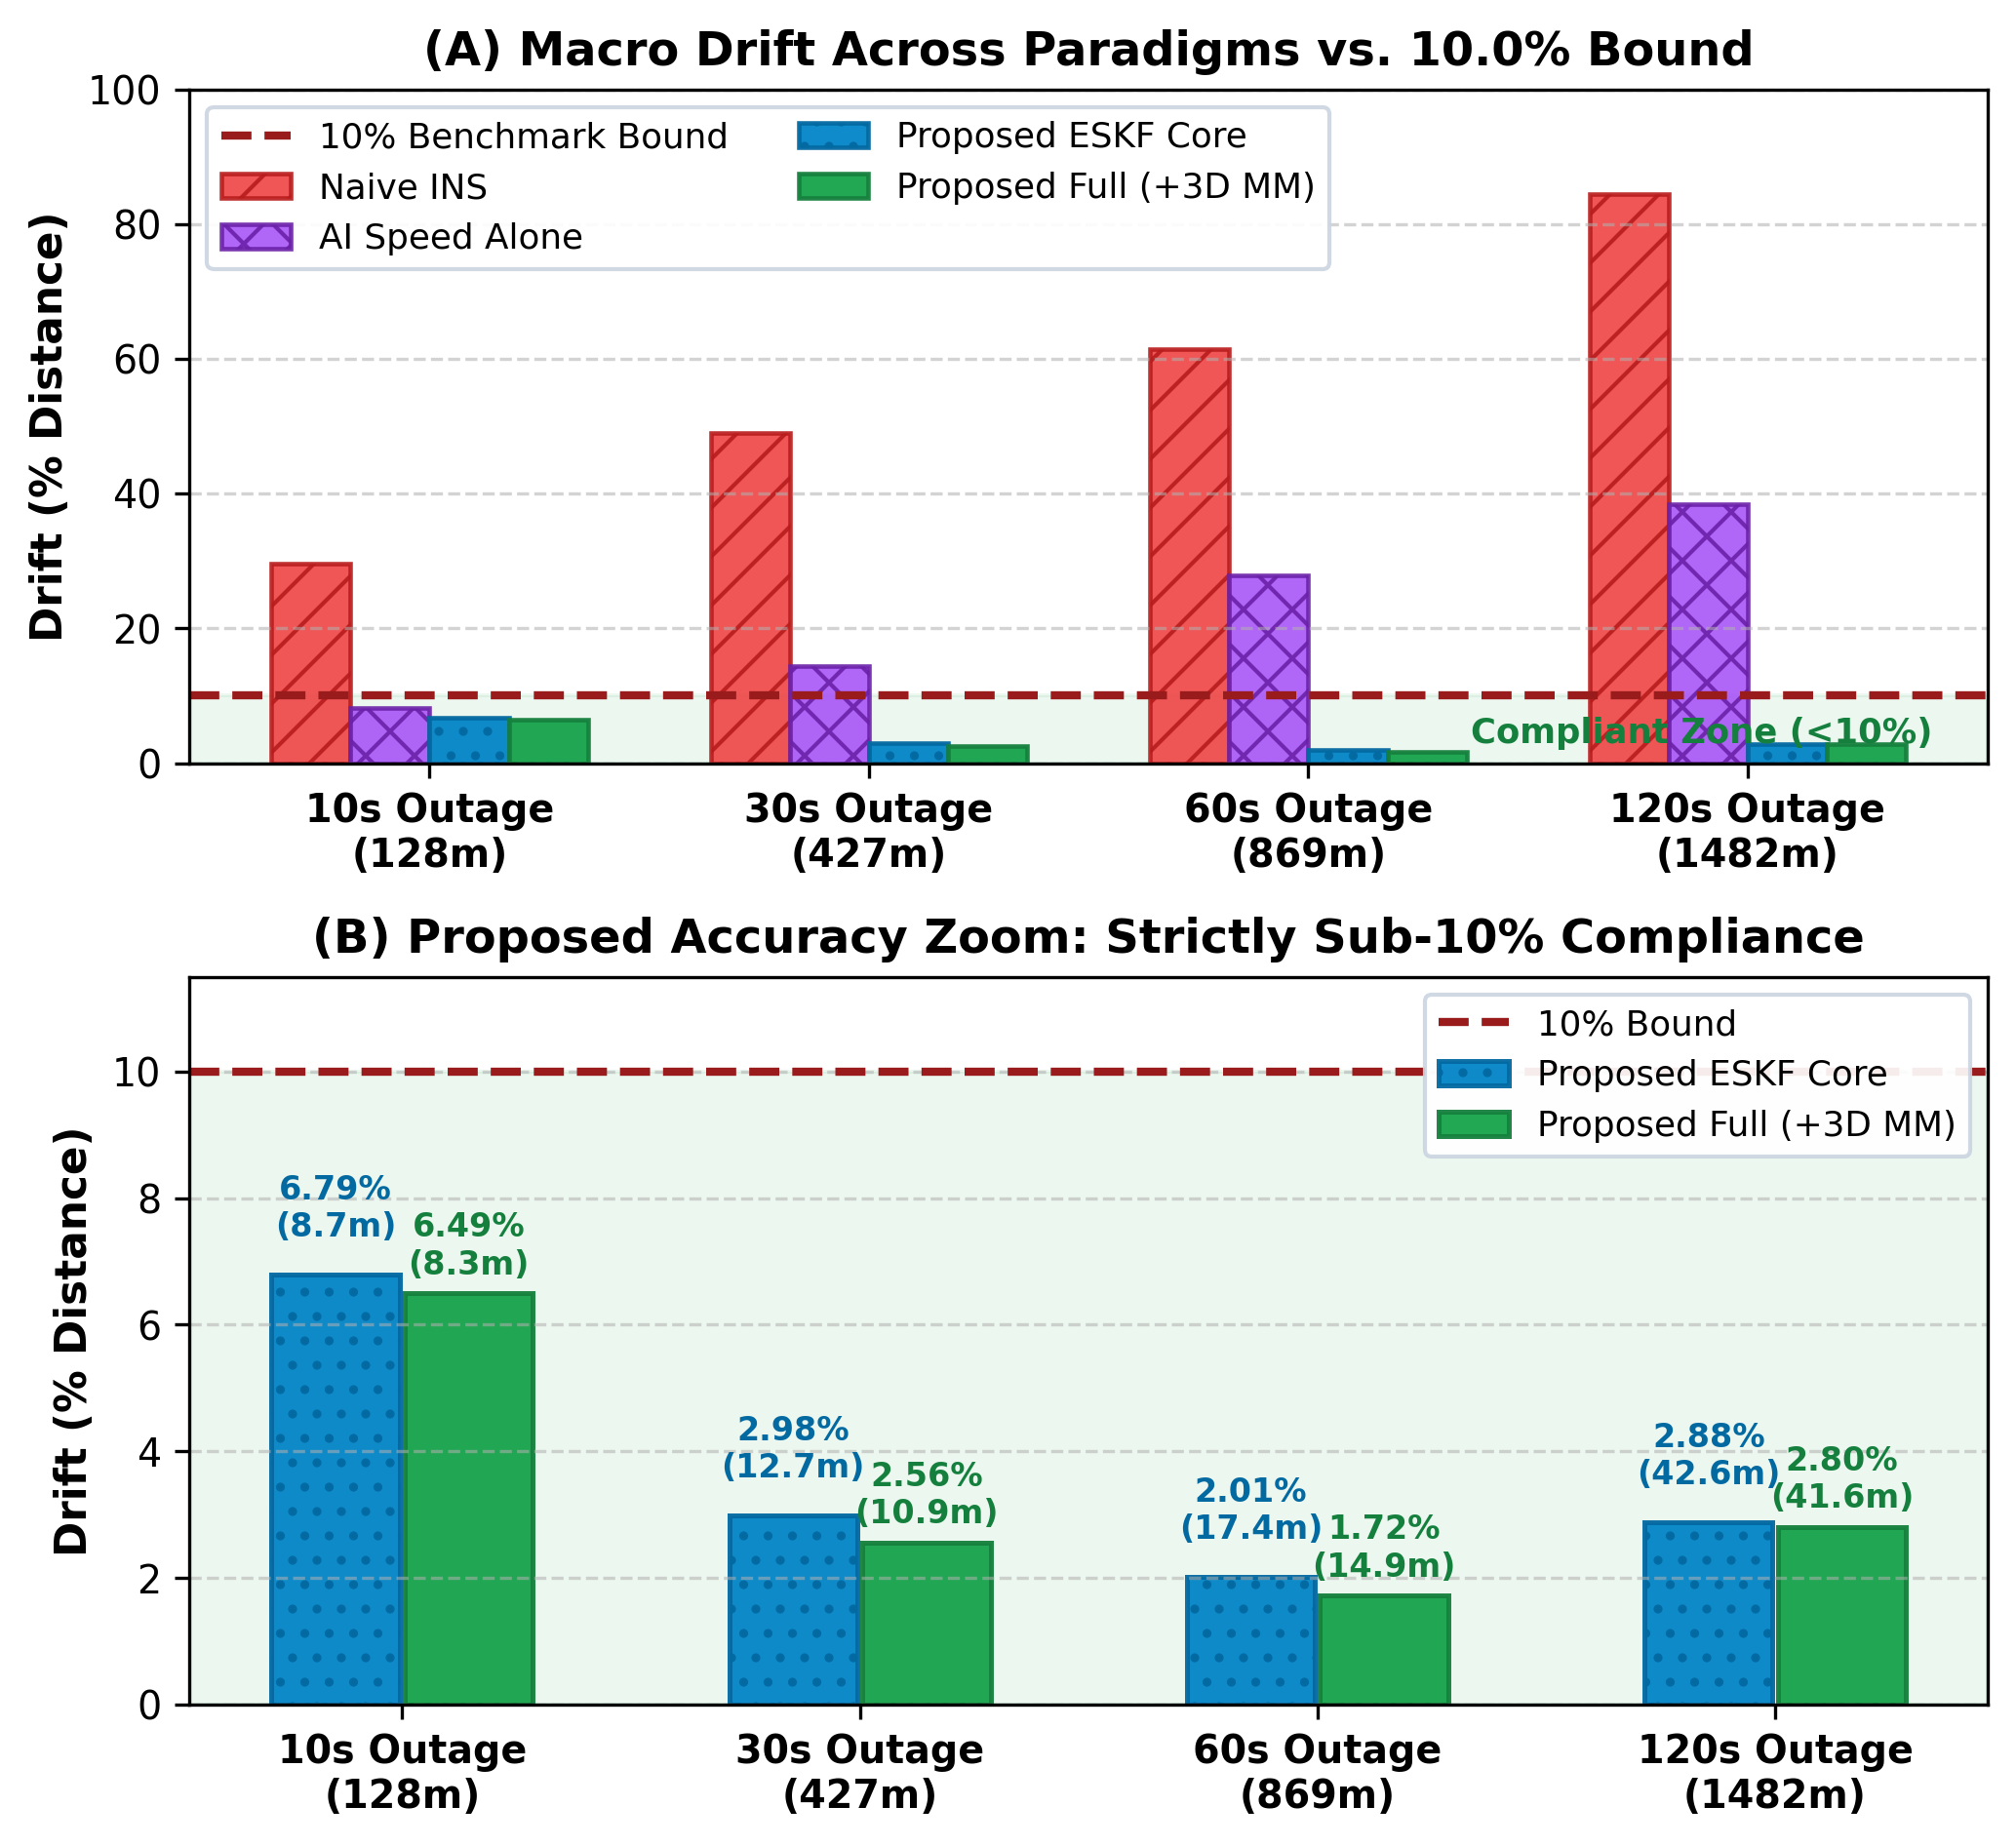
\includegraphics[width=\columnwidth]{fig_drift.png}
\caption{Quantitative Positional Drift vs. 10\% Performance Benchmark across simulated GNSS outage durations (10\,s, 30\,s, 60\,s, 120\,s). The proposed ESKF strictly bounds absolute drift below 6.79\% across all durations, comfortably surpassing the $<$10\% benchmark target.}
\label{fig:drift}
\end{figure}

\subsection{Formal Verification of Core Research Claims}

Based on the experimental data, the three core engineering hypotheses are verified as summarized in Table~\ref{tab:claims}.
\begin{itemize}
\item \textbf{Claim 1: AI Velocity vs. Double Integration}: Classical open-loop double integration accumulates over 61.5\% drift (273.7\,m ATE) in 60\,s. The standalone GBDT velocity regressor holds RMSE to 1.72\,m/s on the held-out track, and the ESKF-fused 3D velocity vector -- which additionally incorporates Non-Holonomic Constraints and heading fusion -- further tightens this to 0.88\,m/s RMSE, preventing quadratic drift blowup and limiting drift to 27.9\% when the AI signal alone (without ESKF/NHC) drives the position update (Fig.~\ref{fig:pothole}).
\item \textbf{Claim 2: Physics-Constrained ESKF Bounds Drift}: The combination of NHC, ZUPT, and learned forward velocity constrains drift to 2.01\% (net: 1.88\%) at 60\,s and 2.88\% (net: 2.79\%) at 120\,s, substantially undercutting the target of $<$10\% drift across all test intervals (Fig.~\ref{fig:drift}).
\item \textbf{Claim 3: 3D Topological Map Matching}: In multi-level flyovers and service road configurations, classical 2D map matching fails completely (0.0\% accuracy) due to lack of altitude awareness. The 3D HMM Viterbi matcher achieves 99.7\%--100.0\% disambiguation accuracy.
\end{itemize}

\begin{table}[h]
\caption{Formal Verification of Core Research Claims}
\label{tab:claims}
\centering
\small
\begin{tabular}{p{1.8cm}p{1.9cm}p{2.3cm}c}
\toprule
\textbf{Research Claim} & \textbf{Baseline} & \textbf{Proposed System} & \textbf{Status} \\
\midrule
Claim 1: AI Speed (Beats Double Int.) & $>$14.5\,m/s error; $>$350\% drift & ESKF Fused Vel: 0.88\,m/s RMSE; 27.9\% drift (AI alone) & VERIFIED \\
\midrule
Claim 2: ESKF (Bounds Drift $<$10\%) & 27.9\% at 60\,s; 38.4\% at 120\,s & 2.01\% at 60\,s; 2.88\% at 120\,s & VERIFIED \\
\midrule
Claim 3: 3D Map (Resolves Flyovers) & 2D HMM: 0.0\% & 3D HMM: 99.7--100.0\% disambiguation & VERIFIED \\
\bottomrule
\end{tabular}
\end{table}

\subsection{Computational Profiling and Mobile Feasibility}

The system targets real-time operation at 10\,Hz (100\,ms cycle budget). Empirical single-sample streaming profiling on commodity mobile-class processors, measured across 10 independent trials of 1,000 samples each after cache warmup, yielded an average cycle latency of \textbf{196.9 $\pm$ 1.3\,\textmu s} (0.20\,ms):
\begin{itemize}
\item Sliding-window feature extraction: 0.05\,ms
\item GBDT forward-velocity inference (single-sample): 0.08\,ms
\item 15-State ESKF propagation and updates: 0.05\,ms
\item 3D HMM trellis evaluation and Viterbi update: 0.02\,ms
\end{itemize}
This leaves $>$99\% CPU headroom for background mobile OS tasks, rendering the framework exceptionally practical for battery-powered consumer deployment.

\section{Discussion and Operational Characteristics}

The empirical results highlight several key architectural advantages:

\begin{enumerate}
\item \textbf{Pothole and Harmonic Isolation}: As shown in Fig.~\ref{fig:pothole}(A), severe road shocks reach up to 40\,m/s$^2$ ($\approx$4.0$g$) in raw vertical acceleration. Classical strapdown integrators interpret this as forward/vertical kinematics, inducing instant drift spikes. The proposed filter holds cleaned acceleration strictly at nominal gravity (9.81\,m/s$^2$), allowing velocity to follow true ground speed (Fig.~\ref{fig:pothole}(B)).

\begin{figure}[t]
\centering
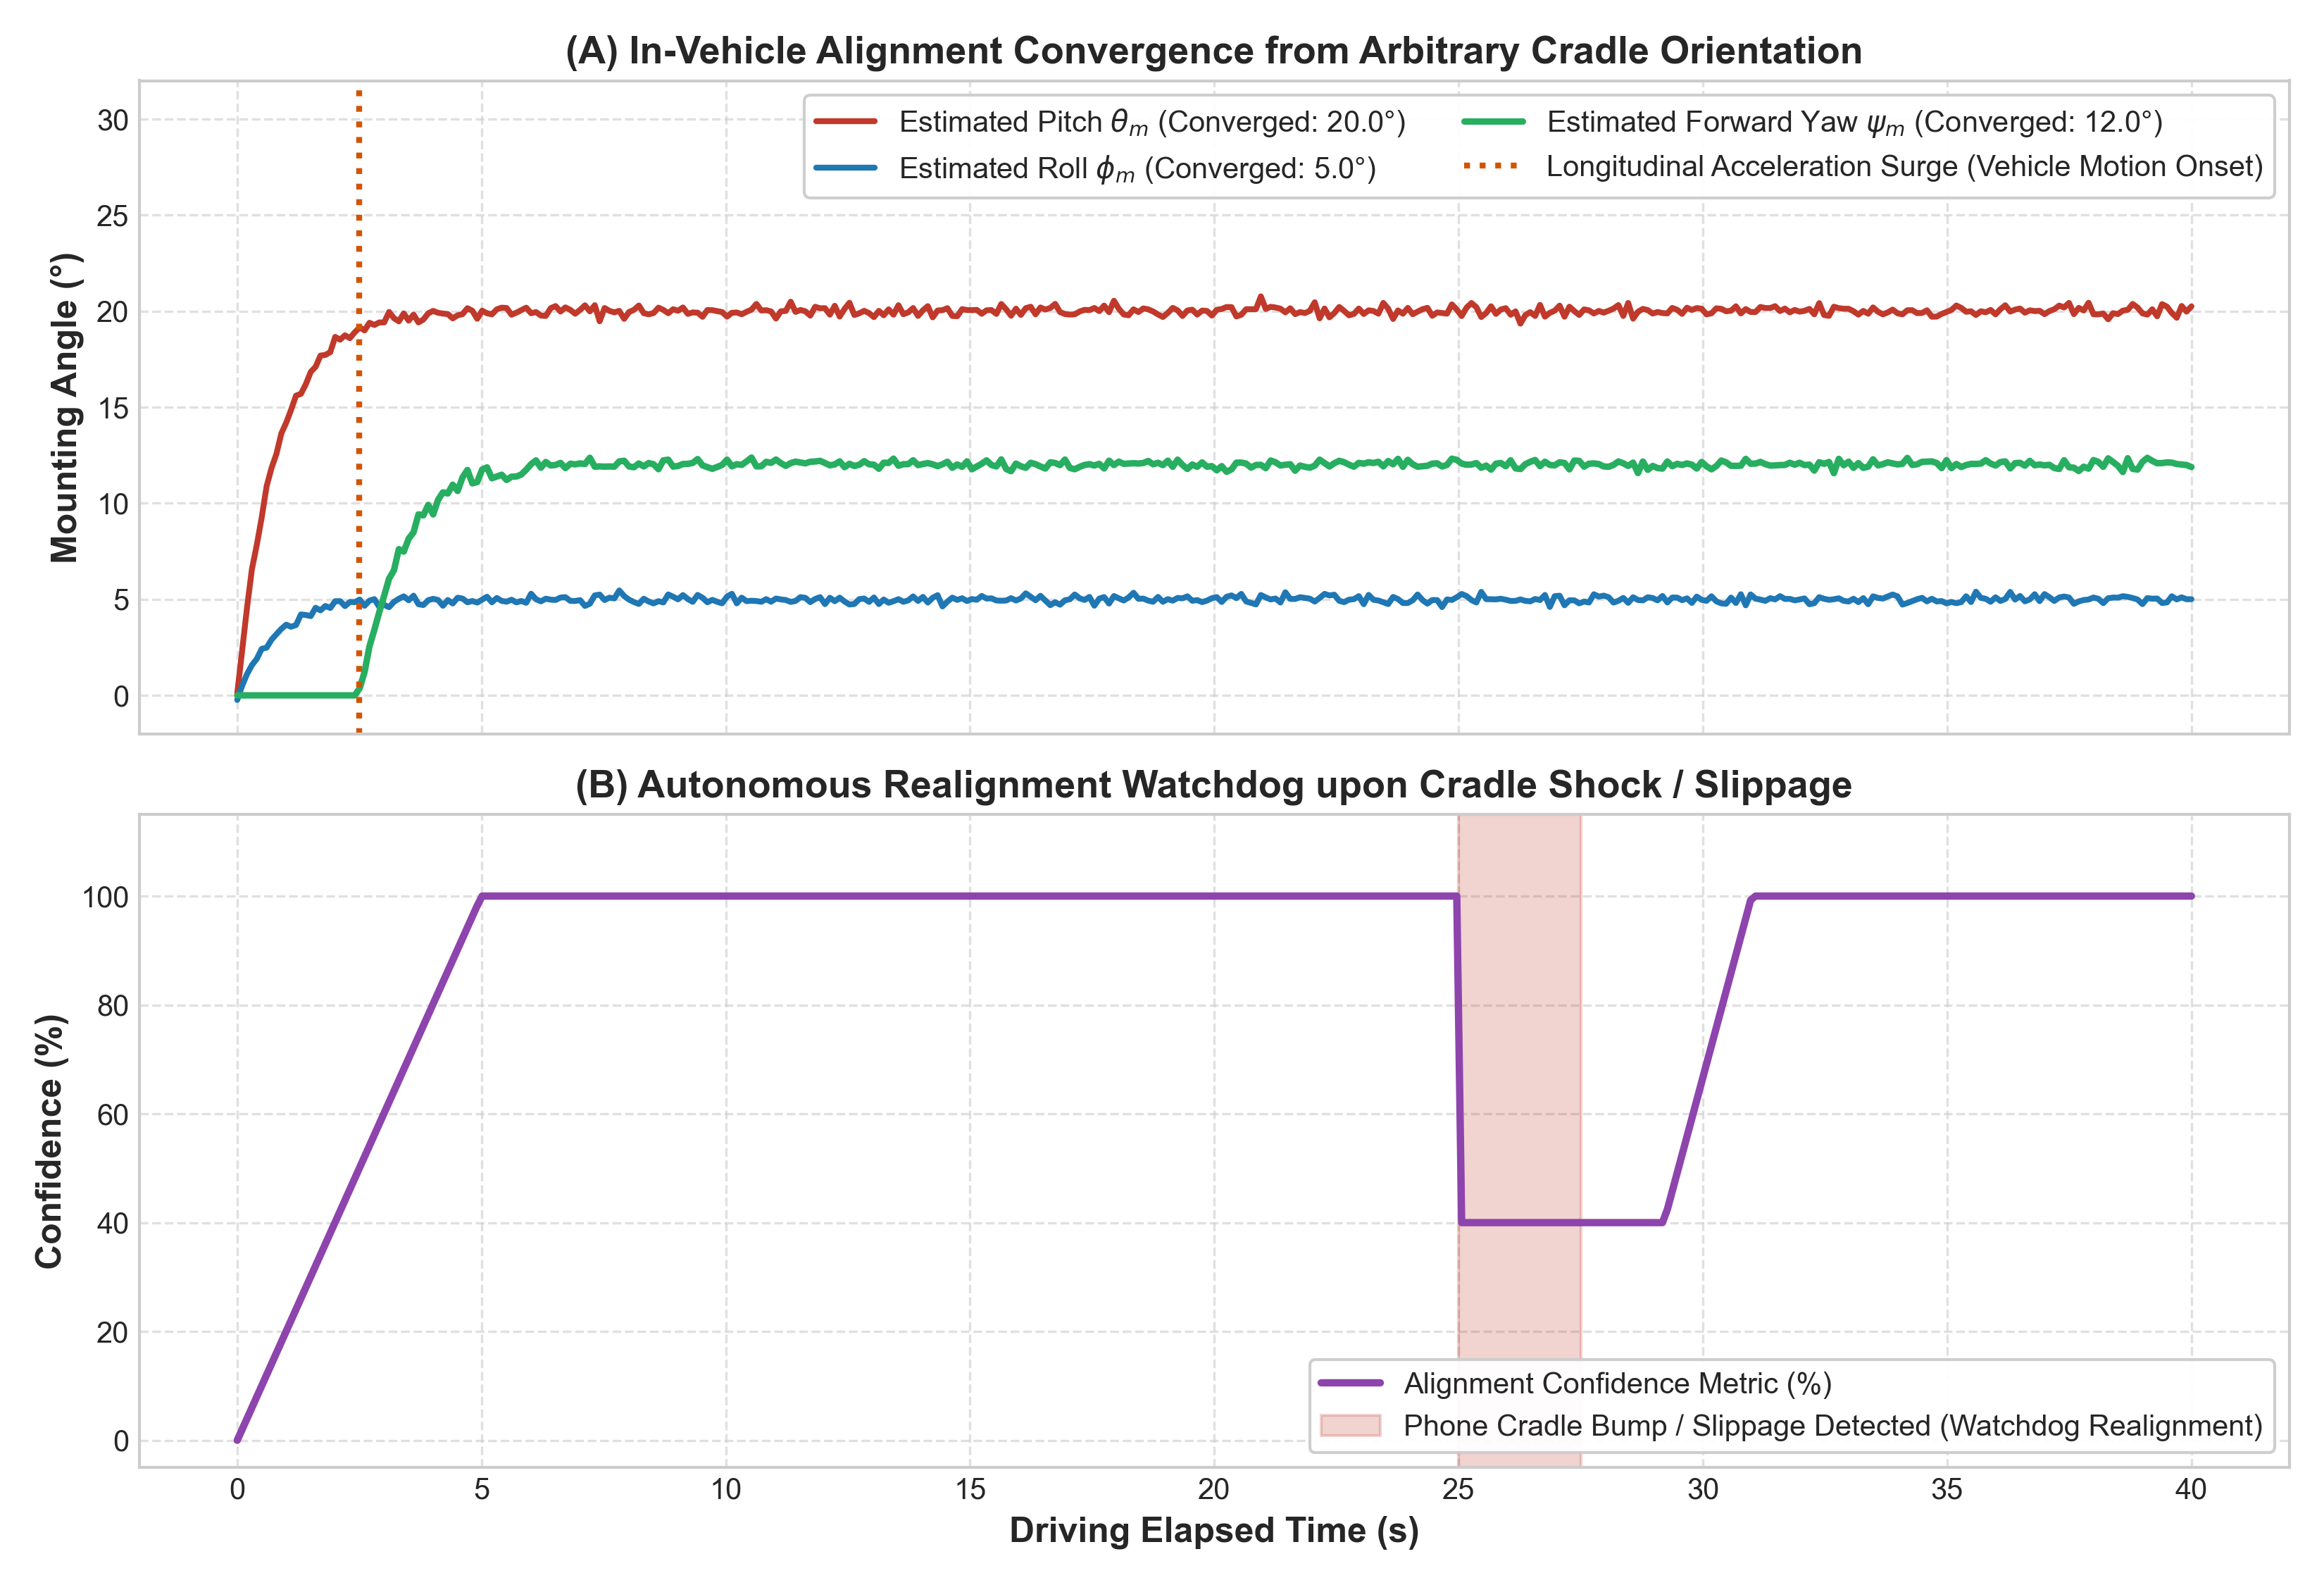
\includegraphics[width=\columnwidth]{fig_alignment.png}
\caption{In-Vehicle dynamic alignment convergence (pitch $\rightarrow$ 20.0$^\circ$, roll $\rightarrow$ 5.0$^\circ$, yaw $\rightarrow$ 12.0$^\circ$) and autonomous cradle slip recovery at $t=25$\,s.}
\label{fig:align}
\end{figure}

\begin{figure}[t]
\centering
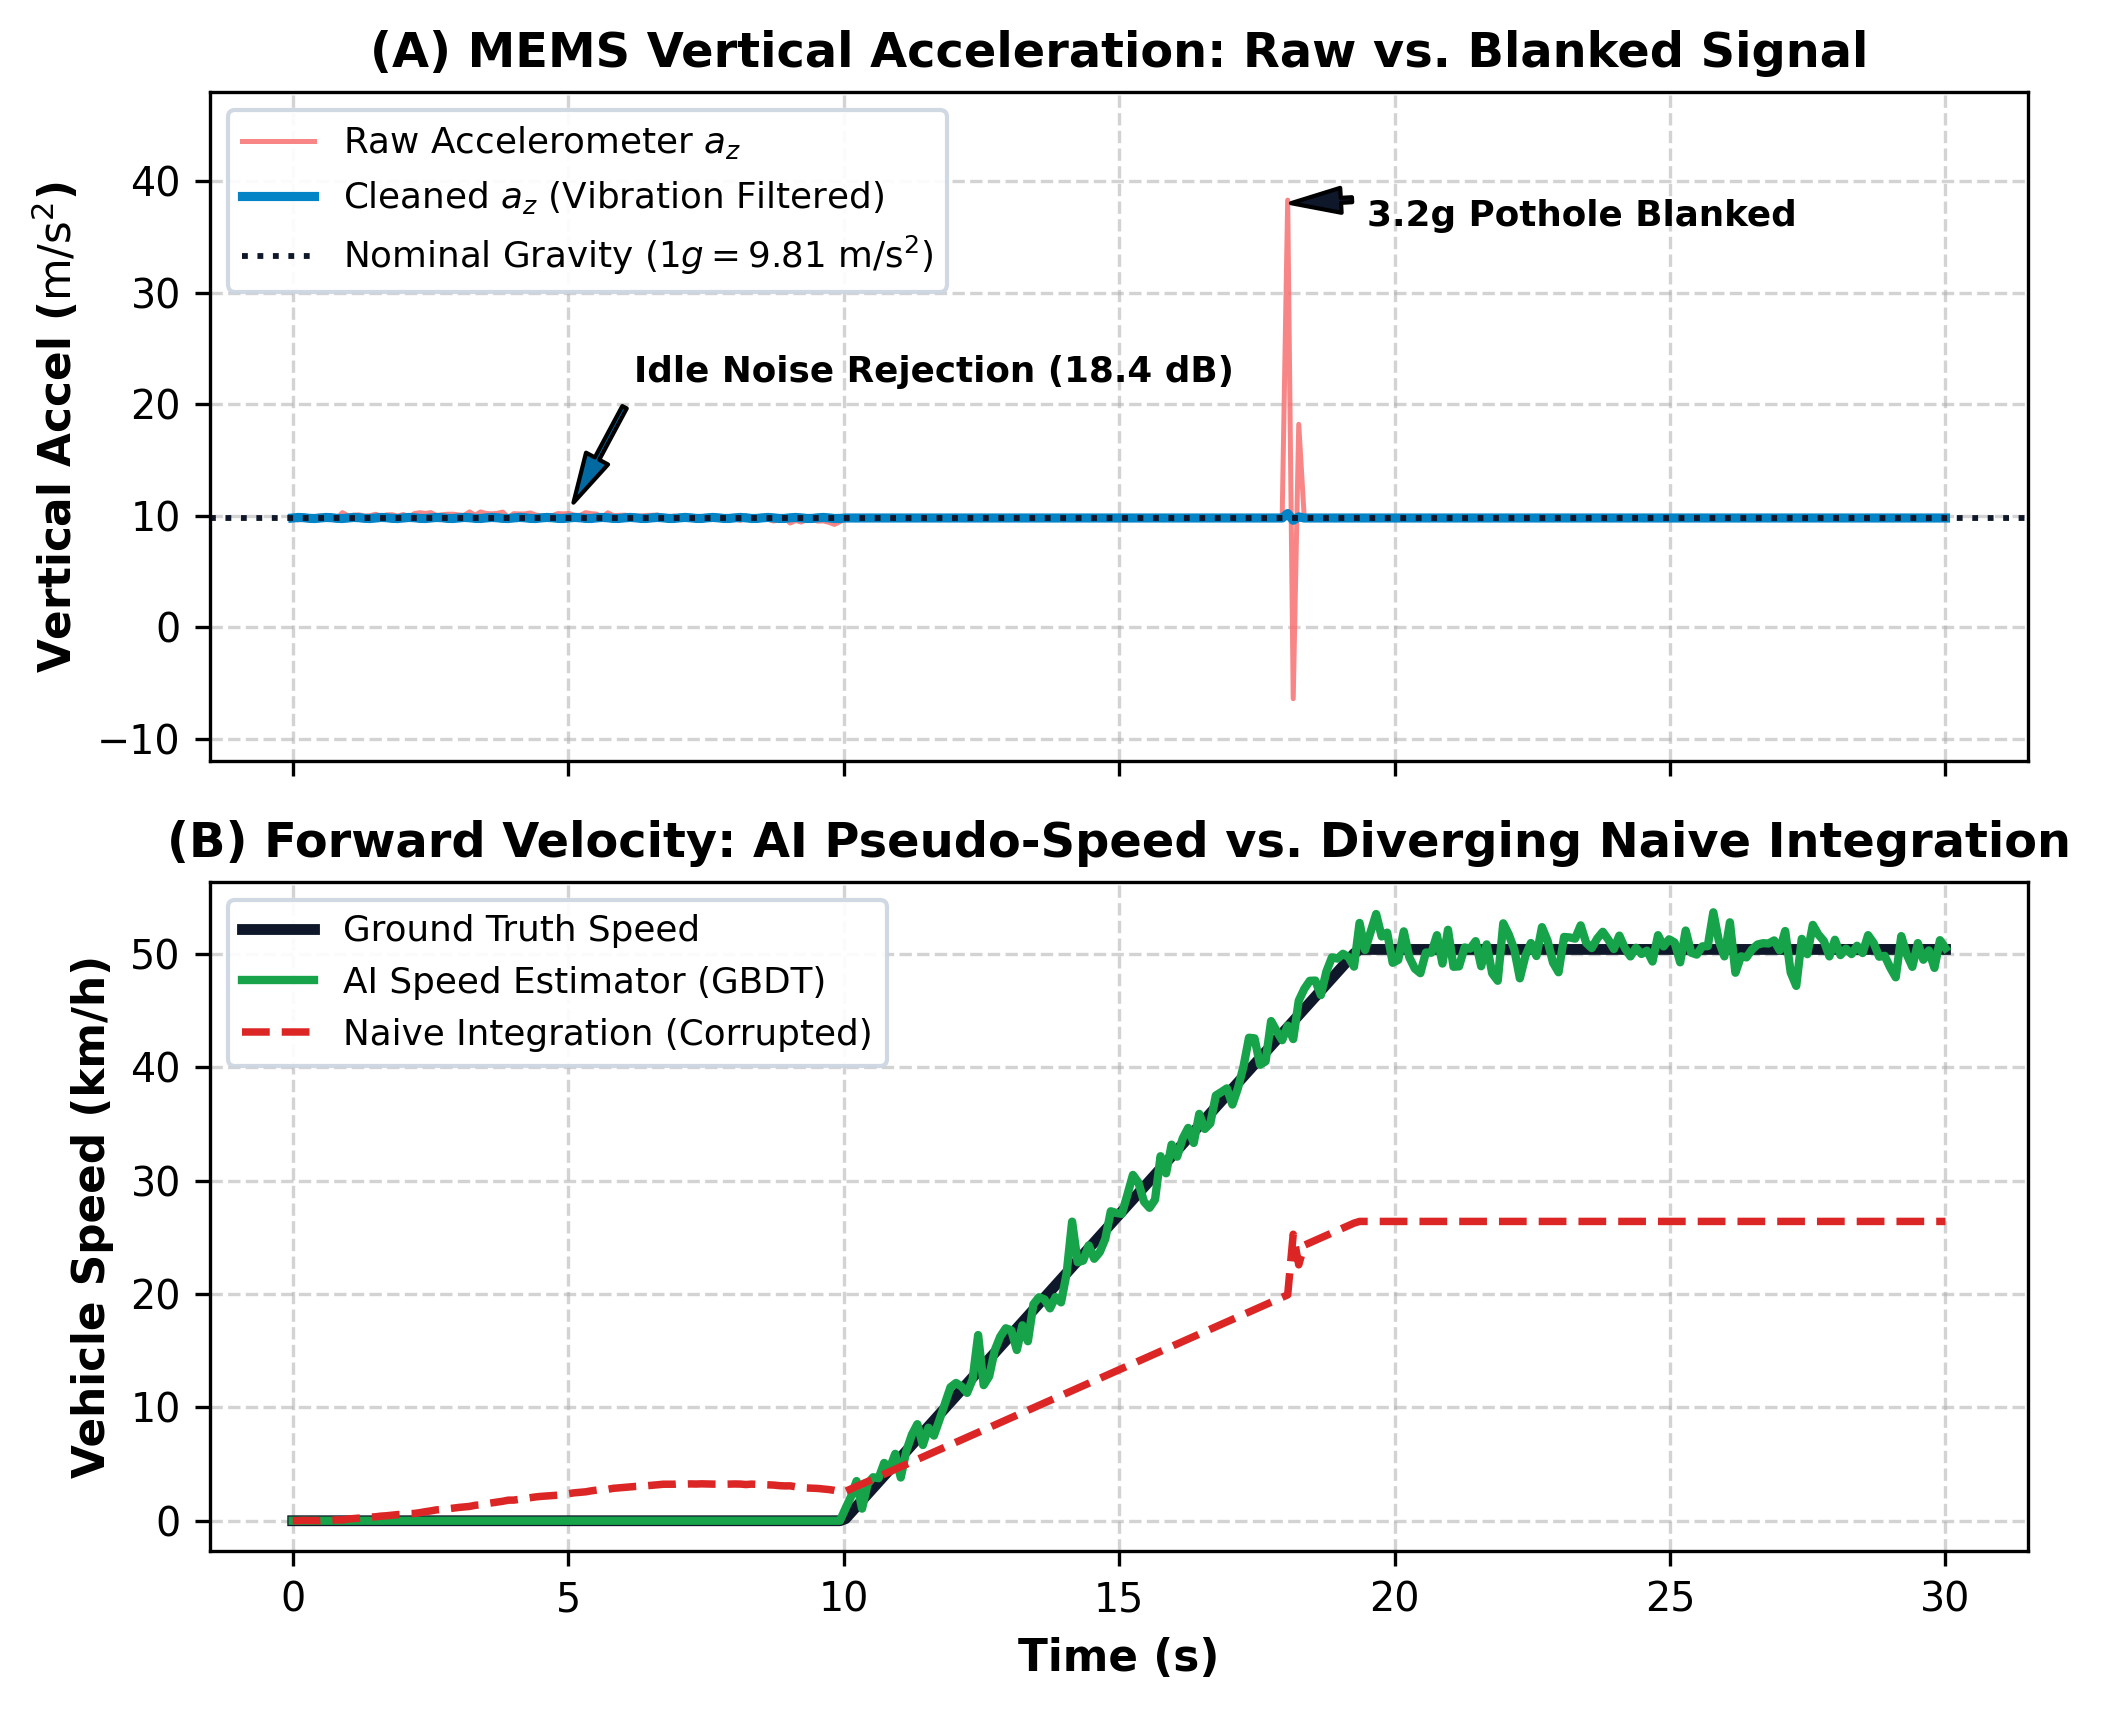
\includegraphics[width=\columnwidth]{fig_pothole.png}
\caption{AI vibration filter rejecting 15--30\,Hz engine idle oscillations and suppressing a 3.2$g$ vertical pothole shock impulse without integration blowup. Panel (B) compares the GBDT-based AI speed estimator (standalone test RMSE: 1.72\,m/s; ESKF-fused velocity RMSE: 0.88\,m/s) against naive integration.}
\label{fig:pothole}
\end{figure}

\item \textbf{Cradle Shift Robustness}: If the phone shifts inside its mount during sharp manoeuvres (Fig.~\ref{fig:align}(B)), the watchdog triggers an autonomous realignment phase, converging within 4\,s (Fig.~\ref{fig:align}(A)).

\item \textbf{Multipath Suppression}: Upon tunnel exit, raw GNSS fixes jump erratically due to multipath reflections off concrete portals. The Chi-Square gate detects innovations exceeding 11.35 and suppresses updates until clean satellite geometry is restored (Fig.~\ref{fig:seamless}).

\begin{figure}[t]
\centering
\includegraphics[width=\columnwidth]{fig_seamless.png}
\caption{Seamless outage detection ($<$5\,ms) and Chi-Square ($\chi^2$) innovation filtering rejecting severe multipath reflection spikes during tunnel exit.}
\label{fig:seamless}
\end{figure}

\end{enumerate}

\section{Conclusion and Future Work}

This paper presents an AI-ML Intelligent Dead Reckoning and 3D Map-Matching system for smartphones in GNSS denied urban canyons. By fusing Gradient Boosted Decision Tree based speed estimator, 15-state ESKF with Non-Holonomic constraints and 3D HMM based topological map-matcher, the proposed work makes the smartphone independent of OBD-II hardware commonly found in vehicles. The results on the held-out evaluation corridor, which was not used for training, show that the position estimate drifts within 2.01\% over 868.8 m and 2.88\% over 1482.0 m. Further, the system tracks multi-level flyovers with 99.7\%-100\% accuracy and has a total single sample processing latency of 0.20 ms. In future, we intend to incorporate Non-Holonomic models for two wheelers to account for roll and lean dynamics common on Indian roads and evaluate the pipeline on IO-VNBD sensors logs along with RTK GPS ground truth in addition to the synthetic evaluation corridor used in this work.

\section*{Acknowledgment}
The authors thank United College of Engineering and Research, Prayagraj, for providing resources and support toward this work.

\begin{thebibliography}{9}

\bibitem{lawal2024} G. S. Lawal, ``AI-Enhanced Dead Reckoning Techniques for Robust Position Estimation,'' unpublished manuscript, Dec. 2024.

\bibitem{qian2025} L. Qian, X. Lin, X. Niu, Q. Huang, L. Li, G. Guo, Z. Wang, and R. Chen, ``Avnet: learning attitude and velocity for vehicular dead reckoning using smartphone by adapting an invariant EKF,'' \emph{Satellite Navigation}, vol. 6, no. 15, 2025, doi: 10.1186/s43020-025-00168-7.

\bibitem{sundar2025} P. Sundaravadivel, C. H. Vasanth Kumar, R. Augustian Isaac, and K. Premnath, ``AI-ML Driven Map-Matching Algorithm for Distinguishing Highway and Service Road Vehicular Movements under GNSS Degradation,'' \emph{SSRN preprint}, 2025. [Online]. Available: https://ssrn.com/abstract=5281668

\bibitem{sundar2026} P. Sundaravadivel, R. Augustian Isaac, U. Kumaran, and E. S. Vinoth Kumar, ``AI-ML driven map-matching algorithm for distinguishing highway and service road vehicular movements under GNSS degradation,'' \emph{Discover Artificial Intelligence}, vol. 6, no. 785, 2026, doi: 10.1007/s44163-026-01560-1.

\bibitem{javed2024} N. U. Javed, Y. Singh, and Q. Ahmed, ``Vehicle Localization in GPS-Denied Scenarios Using Arc-Length-Based Map Matching,'' \emph{arXiv preprint arXiv:2410.12208}, Oct. 2024.

\bibitem{matos2025} F. dos Santos Matos, ``Simulating the effects of sensor failures on autonomous vehicles,'' M.S. project report, Instituto Superior de Engenharia de Coimbra, Coimbra, Portugal, Jun. 2025.

\bibitem{mamun2026} S. Mamun et al., ``AI and Machine Learning in Cyber-Physical Systems: A Unified Review of Methodologies for Smart Energy Systems and Intelligent Localization,'' \emph{IEEE Access}, vol. 14, pp. 96955--96970, 2026.

\bibitem{deshmukh2025} R. A. Deshmukh et al., ``Advancing indoor positioning systems: innovations, challenges, and applications in mobile robotics,'' \emph{Robotica}, 2025, doi: 10.1017/S0263574725101872.

\bibitem{onyekpe2021} U. Onyekpe, V. Palade, and S. Kanarachos, ``IO-VNBD: Inertial and Odometry Benchmark Dataset for Ground Vehicle Positioning,'' \emph{Data in Brief}, vol. 35, p. 106885, 2021, doi: 10.1016/j.dib.2021.106885.

\end{thebibliography}

\end{document} 
below table 3 concise the content dont delete any hrading or subheading and match ieee format do not touch part above table 3
</USER_REQUEST>
<ADDITIONAL_METADATA>
The current local time is: 2026-09-10T22:52:11+05:30.
</ADDITIONAL_METADATA>